\documentclass{article}
\usepackage{setspace}
\doublespacing
\usepackage[utf8]{inputenc}
\usepackage{color}
\usepackage{bm,amsmath}
\usepackage{graphicx}
\bibliographystyle{natbib}
\usepackage{biblatex} %Imports biblatex package
\usepackage{epstopdf}
%\usepackage{natbib}
%\usepackage{centering}
\usepackage{ragged2e} 
%\title{\textbf{Speaker Recognition using Machine Learning: A Study on Efficacy of Gaussian Mixture Models}}
\vspace{-5em}
\title{\textbf{Efficacy of a Gaussian Mixture Model based Speaker Recognition in Machine Learning Framework}}
\author{\textbf{Adhiraj Banerjee}}

%\centering{\Large{4 week report}}
%(SRFP Application No. : ENGS589)

%\date{18 July 2021}

\begin{document}
\vspace{-3em}
\maketitle
\thispagestyle{empty}
%\centering{\textbf{Dr. Siva Ram Krishna Vadali}\\ Senior Principal Scientist \\ Robotics \& Automation Division, CSIR-CMERI Duragpur}
%\centering{August 2021}
\vspace{-3em}
\begin{center}{\textbf{Dr. Siva Ram Krishna Vadali}\\ Senior Principal Scientist \\ Robotics \& Automation Division\\ 
CSIR-Central Mechanical Engineering Research Institute, Durgapur\\}
%\vpsace{1em}
%{August 2021}
\end{center}
\vspace{1em}
\begin{center}{\textbf{August 2021}}
\end{center}
\newpage
\tableofcontents
\newpage
\listoffigures
\newpage
\listoftables
\newpage
\section{\textbf{{Introduction}}}
\label{Intro}
%The topic for my Internship which was assigned to me by my guide is, \textit{Speaker Recognition or Identification using Machine Learning}. Here, the problem I have to solve is that I have to create a trained model which will be able to recognize the speaker from its voice sample provided to it as its input. 
\textcolor{black}{Speech Recognition is a \textit{text-dependent} method, where it highly depends on the language and corpus. On the other hand, Speaker Recognition mainly focusses on raw audio percepts (and from the information derived therein) %by which it identifies the 
to identify the uniqueness aspect, if any, among different speakers \cite{1}. Speaker Recognition (SR) has numerous applications such as voice biometric, forensics, traitor finding, voice-mail and  tele-banking \cite{2}}. Conceptually, SR determines \textcolor{black}{the presence of the active speaker} among a set of registered speakers. %The present work studies available methods for speaker recognition. Further, 
{In view of the applicability of {Machine Learning} framework to a wide variety of classification problems,  \textcolor{black}{the present work studies the popular Gaussian Mixture Model (GMM) based ML (GMM-ML) \cite{3}} approach as a potential solution for speaker recognition. In this work, voice samples of ten different speakers are recorded and the performance of GMM-ML for SR is analyzed. \textcolor{black}{Further, performance of GMM-ML is also studied for SR when the speech samples under test is overlaid with additive white Gaussian noise.} It is observed that GMM-ML based SR is fairly accurate in distinguishing the correct speaker from the $10$ registered speakers. 

\textcolor{black}{The rest of the report is organized as follows: Section \ref{MLforSR} discusses ML for speaker recognition. In this section, GMM-ML using expectation maximization (EM) is studied in detail. Section \ref{result} presents the results and inferences on speaker recognition accuracy using GMM-ML for voice samples. Section \ref{conclusion} provides a few conclusive remarks on the work done.}

\section{\textbf{{Machine Learning for Speaker Recognition}}}
\label{MLforSR}
% \textit{Machine Learning} is a method which helps systems to learn from the training data so that they can predict the class of the test data given as input, without being explicitly programmed for this purpose. This same method would be applied in the Speaker Recognition System. Using Machine Learning, a model for Speaker Recognition will be trained in such a way that it will be able to identify unique patterns and features from different voice samples and distinguish a voice sample from the rest. This method can be applied by, firstly \textbf{gathering different people's speech samples}, \textbf{extract features from the voice sample} suitable for the classifier, which is \textbf{trained for building a trained model} and finally,\textbf{performing classification for recognition of each Speaker} from its corresponding input voice sample.
 \textcolor{black}{\textit{Machine Learning} (ML) is a mathematical framework which helps systems to learn and train a model with (preferably) large data sets and subsequently predict the category into which a test data may be classified to \cite{4}.} 
%Without being explicitly programmed for this purpose. 
 \textcolor{black}{The present work studies the efficacy of a ML based classification algorithm for Speaker Recognition. Going by principles of ML}, a model for Speaker Recognition \textcolor{black}{is trained such that the model identifies unique patterns (referred as features) from a set of different voice samples (of registered speakers) and distinguish the actual speaker voice sample from the rest.} \textcolor{black}{In the present work, Gaussian Mixture Model (GMM) based classification, one of the popular ML methods, is chosen to study its efficacy in accurate speaker recognition.}
% classification 
 %This method can be applied by, firstly {gathering different people's speech samples}, {extract features from the voice sample} suitable for the classifier, which is {trained for building a trained model} and finally,{performing classification for recognition of each Speaker} from its corresponding input voice sample.
\subsection{Gaussian Mixture Model based SR} 
\textcolor{black}{It is known that the Gaussian Mixture Model (GMM) is a 
%statistical 
powerful model used to solve clustering based classification problems.  
%which is 
%formed by 
It is a probabilistic approach as it approximates the probability distribution of a $M X K$ length data ($M$, $K$ dimensional data vectors, where $M$ is number of data points) belonging to a class $\lambda$ (of $L$ possible classes) as a linear combination of $ N$ Gaussian distributions or clusters %the $i^{th}$ %distribution random variable 
with mean vector $\bm \mu$$=$$\{\mu_i\}_{i=1,2,\ldots,N}$ (each of order $K$$X$$1$), variance-covariance \textcolor{black}{matrix} %$\bm \Sigma^\prime$$=$
$\bm \Sigma^\prime$$=$$\{\bm\Sigma_i\}_{i=1,2,\ldots,N}$ (each of order $K$$X$$K$) and $\bm \omega$$=$$\{\omega_i\}_{i=1,2,\ldots,N}$  as the weights in the linear combination.} \textcolor{black}{In 
%case of (each of order $M$$X$$1$)
\textit{Speaker Recognition}, features of speaker's voice sample 
%which are 
are extracted into a feature vector and used as data points for processing to identify the registered speaker. % to compute the likelihood. %in each model till it is maximized. 
Since the feature vector is \textit{multi-dimensional}, %the likelihood 
the probability density function (PDF) 
%also referred as the likelihood, of a given $N$ dimensional feature vector 
of particular class of speaker ($\lambda$, of $L$ possible speakers) can be expressed as a linear combination of $N$ multivariate Gaussian PDFs \cite{5} as:
\begin{equation}
P(\bm X\vert\lambda) = \sum\limits_{i=1}^N \omega_i \cdot P(\bm X|\bm \mu_i,\bm \Sigma_i)
\label{eq1},
\end{equation}
where,
\begin{equation}
P(\bm X|\bm \mu_i,\bm \Sigma_i) = \prod\limits_{n=1}^{M} P(\bm x_n|\bm \mu_i,\bm \Sigma_i);
\end{equation}
%where, \textcolor{red}{$M_i$ denotes the number of data points assigned to the $i^{th}$ Gaussian random variable such that $\sum_{i=1}^N {M_i}$ $=$ $M$};
 %Gaussian random variables used for $N$ clusters formed from the input vector $\bm X$; 
\textbf{$\lambda$}, as mentioned earlier, is the class to which a speaker is associated with; $\bm X$ represents the $N$ dimensional training data; and $P(\bm x_n|\bm\mu_i,\bm\Sigma_i)$ is the multivariate Gaussian PDF given by,%for the $i^{th}$ gaussian distribution.
\begin{equation}
P(\bm x_n|\bm\mu_i,\bm\Sigma_i) = \left({{(2\pi)^K\cdot |\bm\Sigma_i|}}\right)^{-\frac{1}{2}}\cdot exp\left({-\frac{1}{2} (\bm x_n-\bm\mu_i)^T\bm\Sigma_i^{-1}(\bm x_n- \bm \mu_i)}\right).
\label{eq1}
\end{equation}
}
\textcolor{black}{In the formulation in Equation \ref{eq1}, the likelihood, computed from the input data points in vector $X$ is assigned to a particular class corresponding to the speaker's GMM. Herein, the mean vectors ($\bm \mu_i$), variance-covariance matrices ($\bm\Sigma_i$) and weights of each of the gaussian components ($\bm \omega_i$) is updated iteratively till the likelihood for the data points (i.e. feature vectors) is maximized, %, i.e., fit them in each cluster of the model to create the trained Gaussian Model accordingly w.r.t the extracted features. 
thereby creaing a trained model with the extracted features. The maximized likelihood will thus be assigned to the class corresponding to the speaker, in turn creating the the classified GMM for the speaker.} 

\subsection{{{Expectation-Maximization (EM)} Algorithm}} In a Gaussian Mixture Model, the mean vector, the covariance matrix and the weights of each Gaussian components required for obtaining the maximum of the log-likelihood function of datapoints is unknown. {E (Expectation) - M (Maximization) \cite{6}} is an iterative statistical algorithm which is used to train GMM by iteratively updating the unknown parameters ($\bm\mu_i$, $\bm\Sigma_i$ \& $\bm\omega_i$) till convergence is achieved.  Consequently, the EM algorithm assumes great significance. The EM algorithm is computed as follows:
%\begin{itemize}
\subsubsection{{Initialization of Unknown Vector Parameter(s)}} First, the mean vector ($\bm\mu_i$), covariance matrix ($\bm\Sigma_i$) and weights ($\bm\omega_i$) for each of the $N$ Gaussian Distributions or clusters are initialized with arbitary values. From these initialized values, the initial log-likelihood is evaluated.
\subsubsection{{Computation of Responsibilities of Gaussian Components}} In Equation \eqref{eq1}, weights $\{\omega_i\}_{i=1,2,\ldots,N}$ can be considered as a prior probabilities for $N$ Gaussian clusters. \textcolor{black}{Next, for each of the $M$ $K$ dimensional vectors (i.e. $K$ dimensional $\bm X$ $=$ $\{\bm x_n\}_{n=1,2,\ldots,M}$'s) data points, their responsibilities\footnote{Responsibilities in the context may be interpreted as "Contributions"} $\{\bm\gamma_i(\bm x_n)\}_{i=1,2,\ldots N}$ are computed for $N$ Gaussian components are determined.} The responsibilities of $M$ data points can be computed as their corresponding \textit{posterior probabilities} from the initialized parameters of their respective Gaussian components using {Bayes' Theorem}:
%\begin{equation}
%\bm\gamma_i(\bm x) = \frac{\bm\omega_i\mathcal{N}(\bm x|\bm\mu_i,\bm\Sigma_i)}{\sum\limits_{j=1}^N \bm\omega_j\mathcal{N}(\bm x|\bm\mu_j,\bm\Sigma_j)}\,where, \bm\omega_i = \frac{\bm M_i}{\bm M}
%\end{equation}
\begin{align}
\bm\gamma_i(\bm x_n) &= \frac{\omega_i \bm{\mathcal{N}}(\bm x_n|\bm\mu_i,\bm\Sigma_i)}{\sum\limits_{j=1}^N \omega_j \bm{\mathcal{N}}(\bm x_n|\bm\mu_j,\bm\Sigma_j)}\,\\
~&\text{and the latest weight for the $i^{th}$ cluster is given by}~\nonumber\\	
\omega_i &= \frac{ M_i}{M},
\end{align}
where $ M_i$ is the effective number of data points assigned to the $i^{th}$ Gaussian cluster and $ M$ is the total number of datapoints for each speaker.
\subsubsection{{Estimation of Vector Parameters}} Next, estimates of the parameters of each of the $N$ Gaussian components are computed again using the current responsibilities of each data vector $\{\bm x_n\}_{n=1,2,\ldots,M}$ for a particular Gaussian component. Mathematically, paramaters of the $i^{th}$ Gaussian components is given by:

\begin{itemize}
\item {Mean Vector ($\bm\mu_i$)}:
\begin{equation}
\bm\mu_i = \frac{\sum\limits_{n=1}^M\bm\gamma_i(\bm x_n)\bm x_n}{\sum\limits_{n=1}^M\bm\gamma_i(\bm x_n)}.
\end{equation}
Note that, for a given speaker the Mean Vector ($\bm\mu_i$) is of the order of $N X K$ .
\item {Covariance Matrix ($\bm\Sigma_i$)}:
\begin{equation}
\bm\Sigma_i = \frac{\sum\limits_{n=1}^M\bm\gamma_i(\bm x_n)(\bm x_n-\bm\mu_i)(\bm x_n-\bm\mu_i)^T}{\sum\limits_{n=1}^M\bm\gamma_i(\bm x_n)}.
\end{equation}
Note that, for a given speaker, a total of $N$ $K X K$ Covariance Matrices ($\bm\Sigma_i$'s) are computed.
\item {Weight Vector ($\bm\omega_i$) of $i^{th}$ Cluster}:
\begin{equation}
\bm\omega_i = \frac{1}{ M}\sum\limits_{n=1}^M\bm\gamma_i(\bm x_n).
\end{equation}
\end{itemize}
Note that, for a given speaker, a total of $N$ weights ($ \omega_i$) are computed for each of the $N$ clusters.

\subsubsection{{Evaluating the Log-Likelihood}} Next, using the parameters estimated for each of the Gaussian components, the log-likelihood of the data points of a given class  / speaker ($\lambda$) is computed, as follows:
\begin{equation}
\ln P(\bm X|\lambda) = \sum\limits_{n=1}^M\ln\sum\limits_{i=1}^N\bm\omega_i\bm{\mathcal{N}}(\bm x_n|\bm \mu_i,\bm \Sigma_i).
\end{equation}
%\end{itemize}
Next, the criteria for convergence in the E-M Algorithm is examined / compared as follows:
\begin{enumerate}
\item If the parameters of the Gaussian components ($\bm\mu_i$,$\bm\Sigma_i$, and $\bm\omega_i$) does not change in the last successive iterations and 
\item If the log-likelihood of the data points for a particular speaker remains almost unchanged in the last few iterations (thereby indicating attaining maxima of the function) 
\end{enumerate}
stop iterating and use the EM computed estimates for further processing (i.e. identification of the speaker in the present application). Note that, if convergence of data points for $N$ Gaussian clusters is not fulfilled, all the steps from the second step need to be repeated. Figure \ref{ML_flow} shows the a schematic of the flow of GMM-ML based speaker recognition. 
 \begin{figure}[h]
\begin{center}
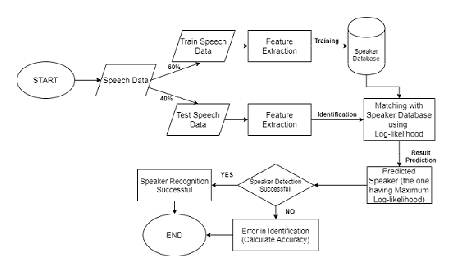
\includegraphics[scale = 2.0]{ML_flow.eps}%{framing}
\caption{Flow chart of GMM-ML based speaker recognition}
\label{ML_flow}
\end{center}
\end{figure}
\subsection{Feature Extraction in SR: Mel-Frequency Cepstrum Coefficients (MFCC)}
The features extracted from the voice samples are referred as \textit{Mel-Frequency Cepstrum Coefficients (MFCC's)} \cite{7}. In the context of audio signal processing, MFCCs have become a prominent feature to be used for feature extraction from train data, because it gives an idea about the perceived difference between frequencies, especially in higher frequency region. Its importance comes from the fact that, the human ear can perceive voice signal frequncies in a \textit{non-linear} fashion. Clearly, for further signal processing, audio frequencies needs to be analyzed in the \textit{Mel} scale, rather than the {Hertz} scale. Moreover, since there is a logarithmic relationship between the Mel and Hertz scale, frequencies in Mel scale becomes more useful. The extraction of MFCCs can be accomplished as explained in the following modules:
%\begin{itemize}
\subsubsection{{Pre-Emphasis}} After discretization of the analog voice signal, since the frequency range where the human ear tends to perceive less in linear scale, first, Pre-Emphasis \cite{8} is performed to increase the energy of the signal at higher frequencies.\footnote{Pre-Emphasis is mainly done for transmission cases which induces the significance of the presence of higher frequency components in the voice signal.} Pre-Emphasis is performed by passing the signal through a \textit{first order high pass filter}. The discrete time equation for filtering the the audio signal (x[n]) and the filtered output signal (y[n]) is given by:
\begin{equation}
{y[n]} = {x[n]} - {\alpha x[n-1]} \, \forall\, {\alpha}\in (0.9,1) 
\end{equation}
The Z-transform of the digital filter is given by:
\begin{equation}
{H(z)} = 1-{\alpha z}^{-1}
\end{equation}
\subsubsection{{Extraction of Frames}} Due to changes in \textit{Prosody} (i.e. features of voice) and \textit{random variations} in the vocal tract, the voice signal is a \textit{non-stationary signal}. However, within short intervals the voice signal is assumed to be \textit{stationary}, and may hence be analyzed over short time windows. Hence, for analysis of voice features, the speech signal is divided into frames of length ${N}$ and {M} samples from adjacent frames are overlapped. Figure \ref{fig1} shows frames to be extracted from a recorded audio / voice signal. 
\begin{figure}[h]
\begin{center}
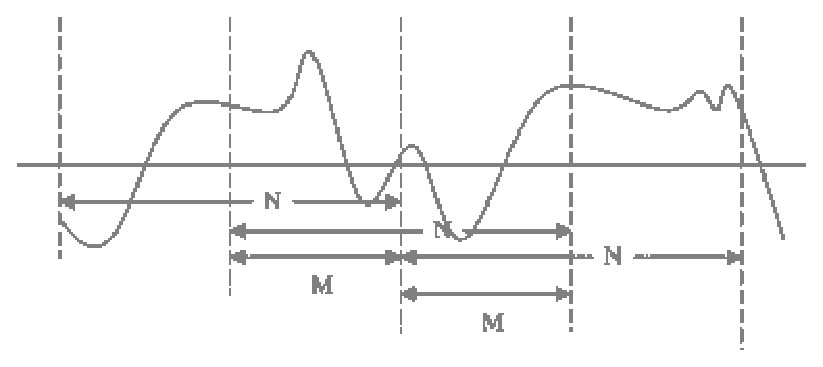
\includegraphics[scale = 0.9]{fig1.eps}%{framing}
\caption{Extraction of frames from voice signal}
\label{fig1}
\end{center}
\end{figure}
\newpage
\subsubsection{{Smoothing voice signals with filters}} When the audio signal is divided into short frames, discontinuities are formed at the edges of the frame, which are incongruent to the input voice signal. Such discontinuities impact the signal by changing its {statistical properties}. In order to reduce the effect, voice signal is smoothened by multiplying each frame with a window, i.e. filtered such that a smoothing behavior is enforced leading to zero signal strength at the borders. Generally, the signal frames are multiplied with the \textit{Hamming Window} \cite{9}. Considering the window to be w[n], the equation for windowing is :
\begin{equation}
y[n] = x[n]\cdot w[n]
\end{equation}
where, ${x[n]}$ is the input signal, ${y[n]}$ is the output signal and for $N$ being the number of samples in each frame,
\begin{equation}
{w[n]} = 0.54-0.46\cdot {\cos{\frac{2\pi n}{N-1}}}\,\forall\,{n\,\in\,[0,N-1]}
\end{equation}

\subsubsection{{Computation of the Fast Fourier Transform (FFT)}} Next, Discrete Fourier Transform (DFT) of each frame is computed to obtain absolute frequency spectrum. Note that, for this $N_1$ point Fast Fourier Transform (FFT) (such that $N_1$ $>$ Sample size of each frame) is computed. The samples of spectrum are considered from $k = 0,1,\dots,$$\frac{N_1}{2}$, spaced at $k\frac{f_s}{N_1}$. Note $f_s$ is the sampling frequency and $k\frac{f_s}{N_1}$ is called resolution. Mathematically, DFT is computed as:
\begin{equation}
{X[k]} = \sum\limits_{n=0}^{N_1-1}{x[n]\cdot \exp{\frac{-j2\pi nk}{N_1}}}\,\forall\, {k}=0,1,.....,{\frac{N_1}{2}}
\end{equation}
where, ${x[n]}$ is the input signal (i.e. frame) and ${X[k]}$ is the FFT of the input x[n]. Finally, ${|X[k]|}$ is the absolute values of the frequency spectrum of frames of the input voice signal.
\subsubsection{{Mel-Filter Bank Processing}} The frequency spectrum is then passed through a Mel-filter bank, which is a bank of triangular filters plotted against frequencies in Mel Scale. The relationship between frequencies in Hz scale and frequencies in Mel-scale can be expressed as:
\begin{equation}
{f}_{Mel} = 2595\cdot\log_{10}{\left(1\,+\,\frac{{f}_{Hz}}{700}\right)}
\end{equation} 

\begin{figure}[!h]
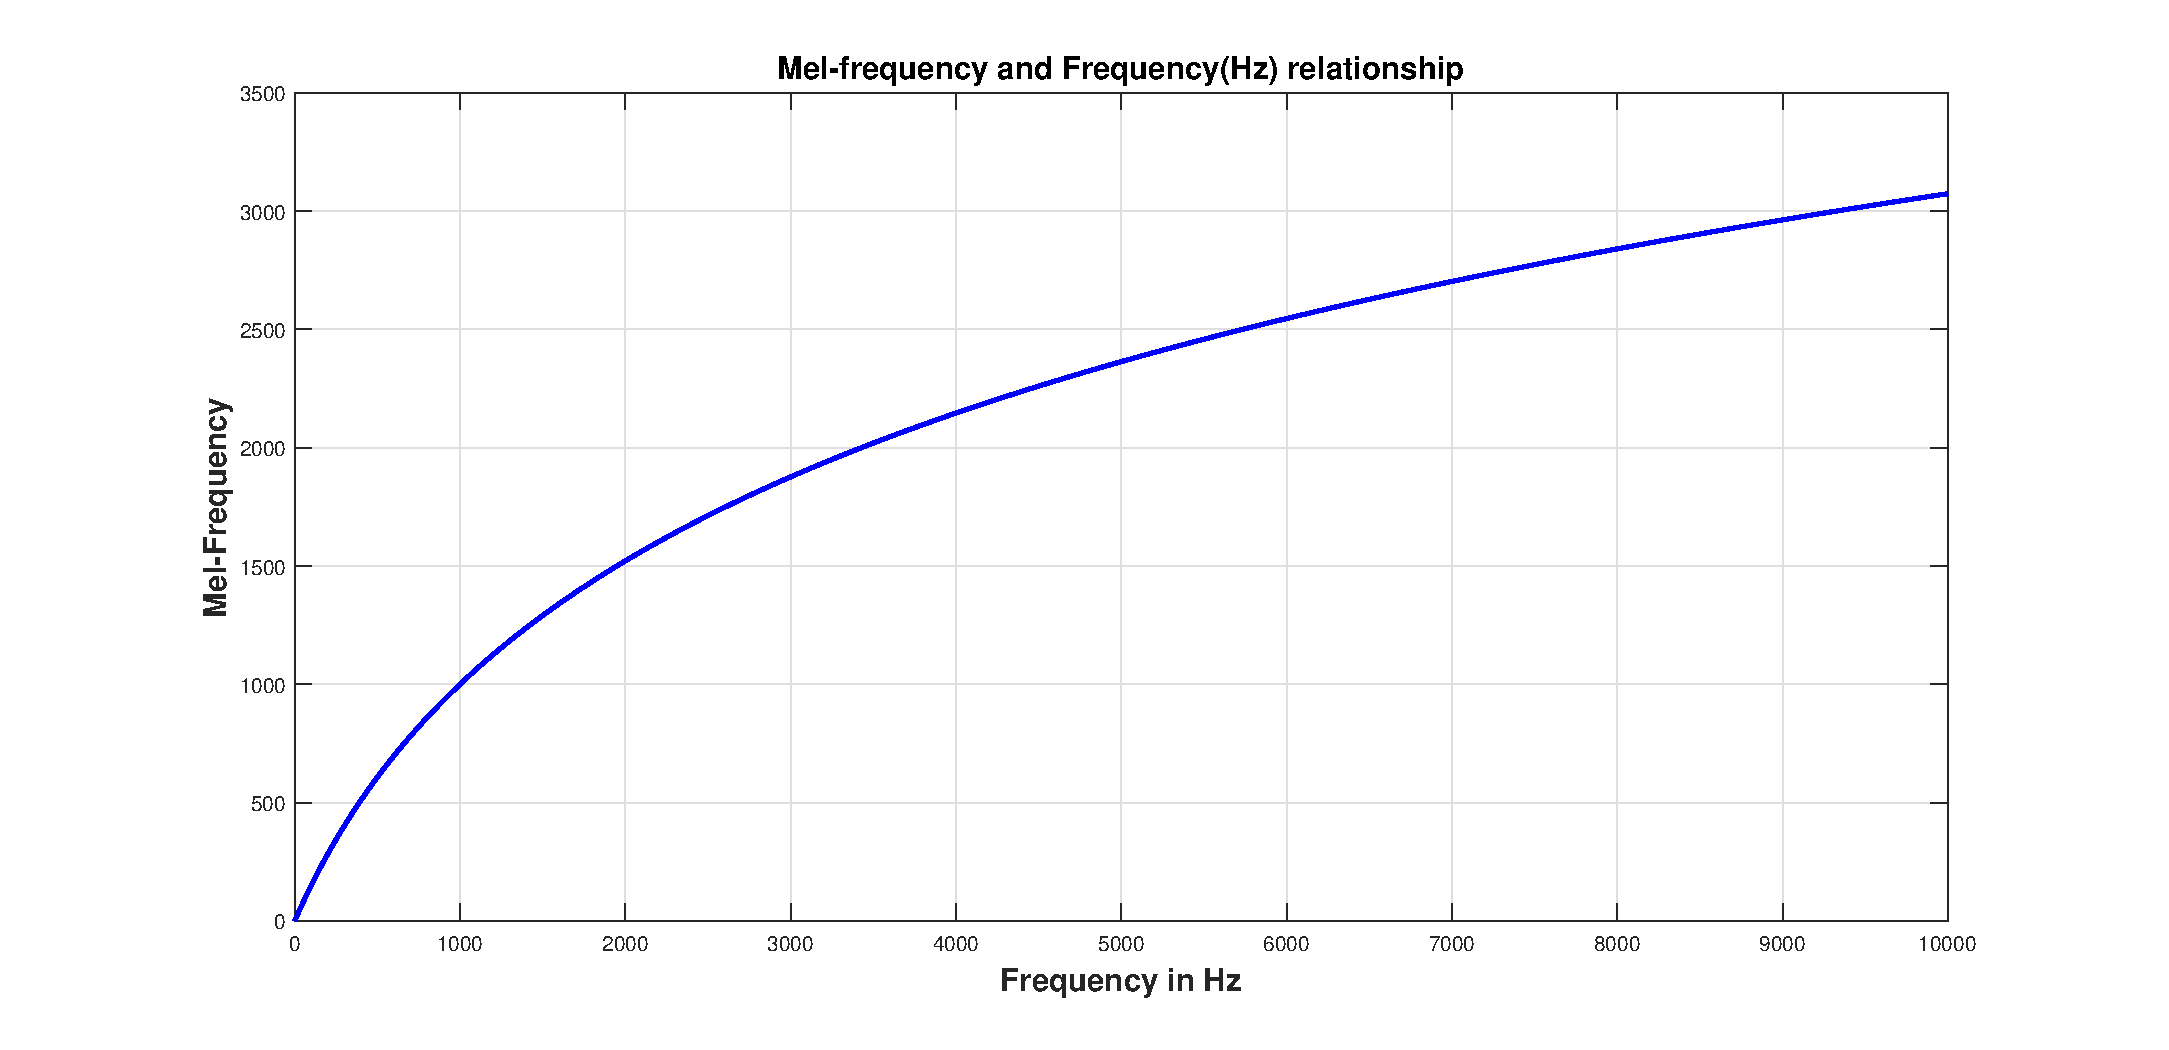
\includegraphics[scale=0.4]{fig2.eps}%{Mel-relation}
\caption{Relationship between Mel-scale and Hz-scale}
\label{fig2}
\end{figure}
%Here, $L$ filters are used within $k$ = $0,...,$$\frac{N}{2}$. 
The output of frequency spectrum after passing throught Mel-filter bank \cite{10} gives the Mel-Frequency spectrum. Figure \ref{fig2} shows the relation between Mel-scale and the Hz scale.  
\begin{figure}[!b]
\begin{center}
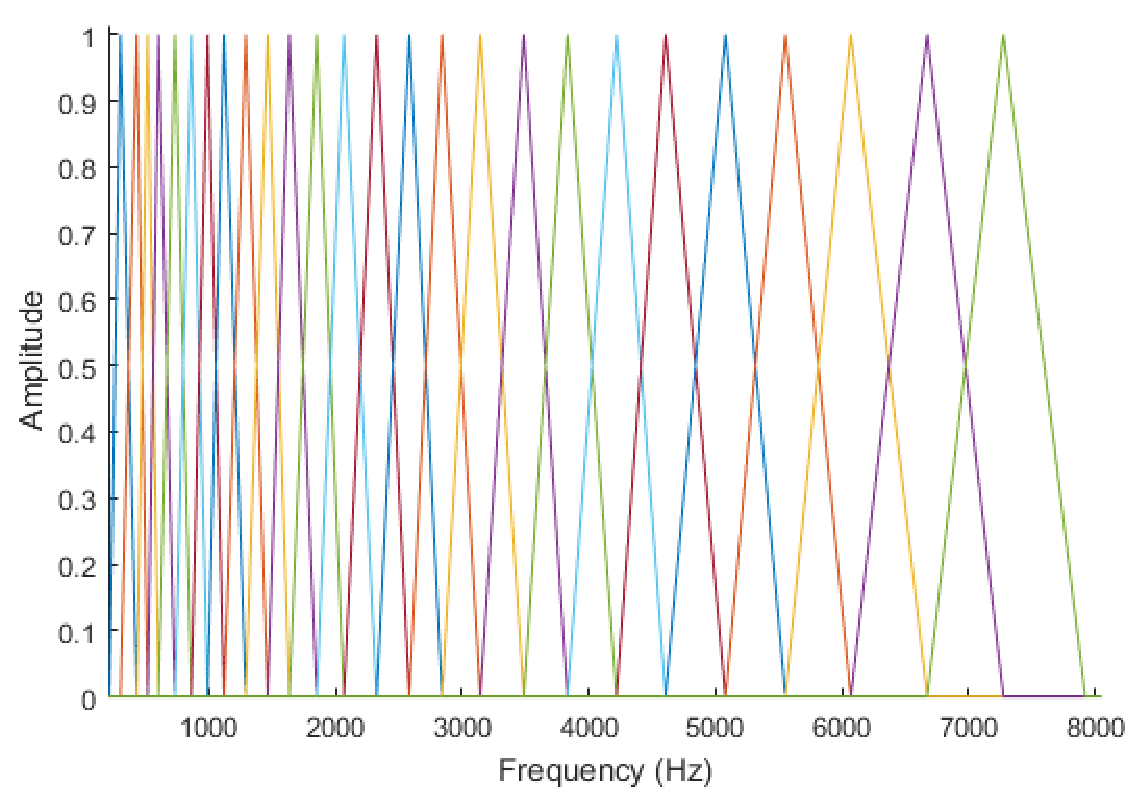
\includegraphics[scale=0.6]{fig3.eps}%{mel_filters}
\caption{Triangular Mel-Filter Bank}
\label{fig3}
\end{center}
\end{figure}
The equation for the filter output $\tilde S(l)$ is given below:
\begin{equation}
{\tilde S(l)} = \sum\limits_{k=0}^{N_1/2}{S(k)\cdot M_l(k)}\,\forall\,\,{l} = 0,1,\ldots,{L}-1
\end{equation}
where, ${S(k)=|X[k]|}$ is the frequency spectrum for the input ${x[n]}$ and ${L}$ is the number of Triangular Mel-filters used for filtering the whole spectrum to obtain the Mel-frequency spectrum. % over the whole range of $k$.
Figure \ref{fig3} shows the triangular Mel filter bank. The spectrum obtained from filtering operation renders non-linear frequency spectrum at the higher frequencies. % which human ear can obtain. This way, though the bandwidth is kept same, the perceived difference between frequencies can also be obtained in all frequency ranges. 
The Mel-filter bank usage is important as voice signal generally follows frequencies in non-linear form and thus the human ear can perceive frequencies being non-linear.


\subsubsection{{Conversion of Mel-Spectrum to Mel-Cepstrum}} The logarithm of the Mel-frequency spectrum is taken to obtain Mel-Frequency Cepstrum. Figure \ref{fig4} shows the conversion of spectrum to cepstrum.  
\begin{figure}[h]
\begin{center}
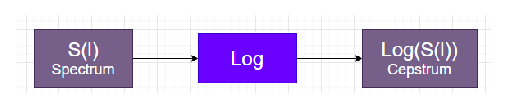
\includegraphics[scale=1.5]{fig4.eps}%{Cepstrum}
\caption{Conversion of spectrum to cepstrum}
\label{fig4}
\end{center}
\end{figure}
\subsubsection{{Computation of MFCCs}} As a last step, the MFCC coefficients are obtained by computing the Discrete Cosine Transform (DCT) of the Cepstral coefficients obtained in previous step. %, is operated upon by taking its \textit{Discrete Cosine Transform(DCT)} which provides us MFCCs as the final result. 
Mathematically, DCT is computed as follows:
\begin{equation}
{c(i)} = \sqrt{\frac{2}{L}}\sum\limits_{m=1}^L{\log{(\tilde S(m))}\cdot \cos{\left(\frac{\pi i}{L}(m-0.5)\right)}}\,\forall\,{c}=0,1,\ldots,{C}-1
\end{equation}
where, ${C}$ is number of desired MFCCs, ${\log{(\tilde S(m))}}$ is the Mel-Cepstral coefficients and ${L}$ is the number of triangular mel-filters used for obtaining the Mel-spectrum.
%\end{itemize}

\section{\textbf{{Experimental Results and Observations}}} 
\label{result}
In the present work, 
%From the results after testing the related python codes, 
GMM based Speaker Recognition is tested for its efficacy over $10$ speakers. The entire coding is done in a Python environment. %\section{\textbf{Observations in accuracy of GMM in SR for Speech samples with noise}}
As discussed in the foregoing discussion, first the features are extraced from the training of speech files and the Gaussian Mixture Models (GMM) are trained. It has been observed that, for the speech samples which were recorded and stored for training and testing purpose render highly accurate results, i.e. atleast 100\% approx. for chosen $10$ speakers.

%
%\begin{figure}[!h]
%\begin{center}
%\includegraphics[scale=0.4]{audio.eps}%{Cepstrum}
%%
\includegraphics[scale=0.4]{Audio_Case-2.eps}%{Cepstrum}
%%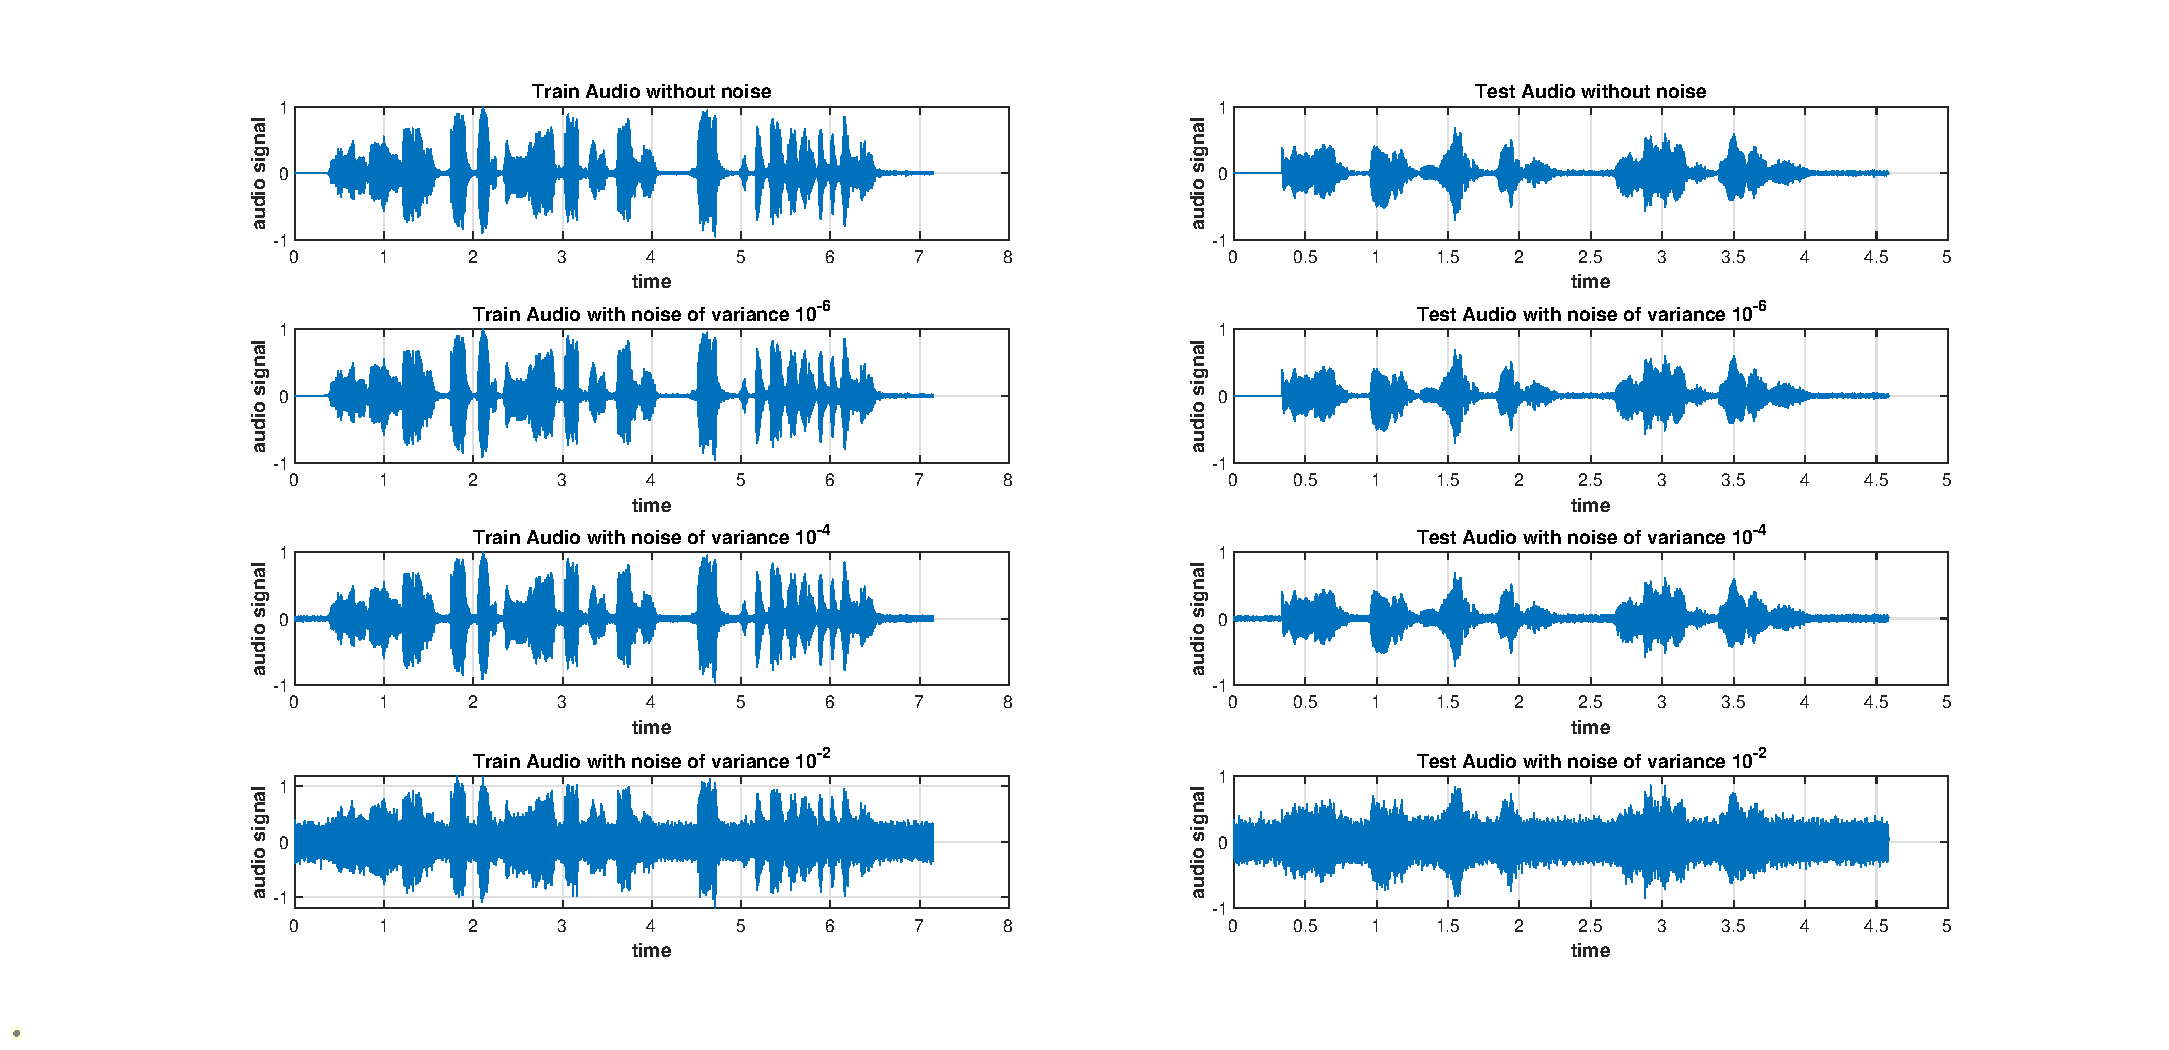
\includegraphics[scale=0.4]{Audio_Case-3.eps}%{Cepstrum}
%\caption{Conversion of Spectrum to Cepstrum}
%\end{center}
%\label{audiofiles}
%\end{figure}
%
%\begin{figure}[!h]
%\begin{center}
%%\includegraphics[scale=0.4]{audio.eps}%{Cepstrum}
%
\includegraphics[scale=0.4]{Audio_Case-2.eps}%{Cepstrum}
%%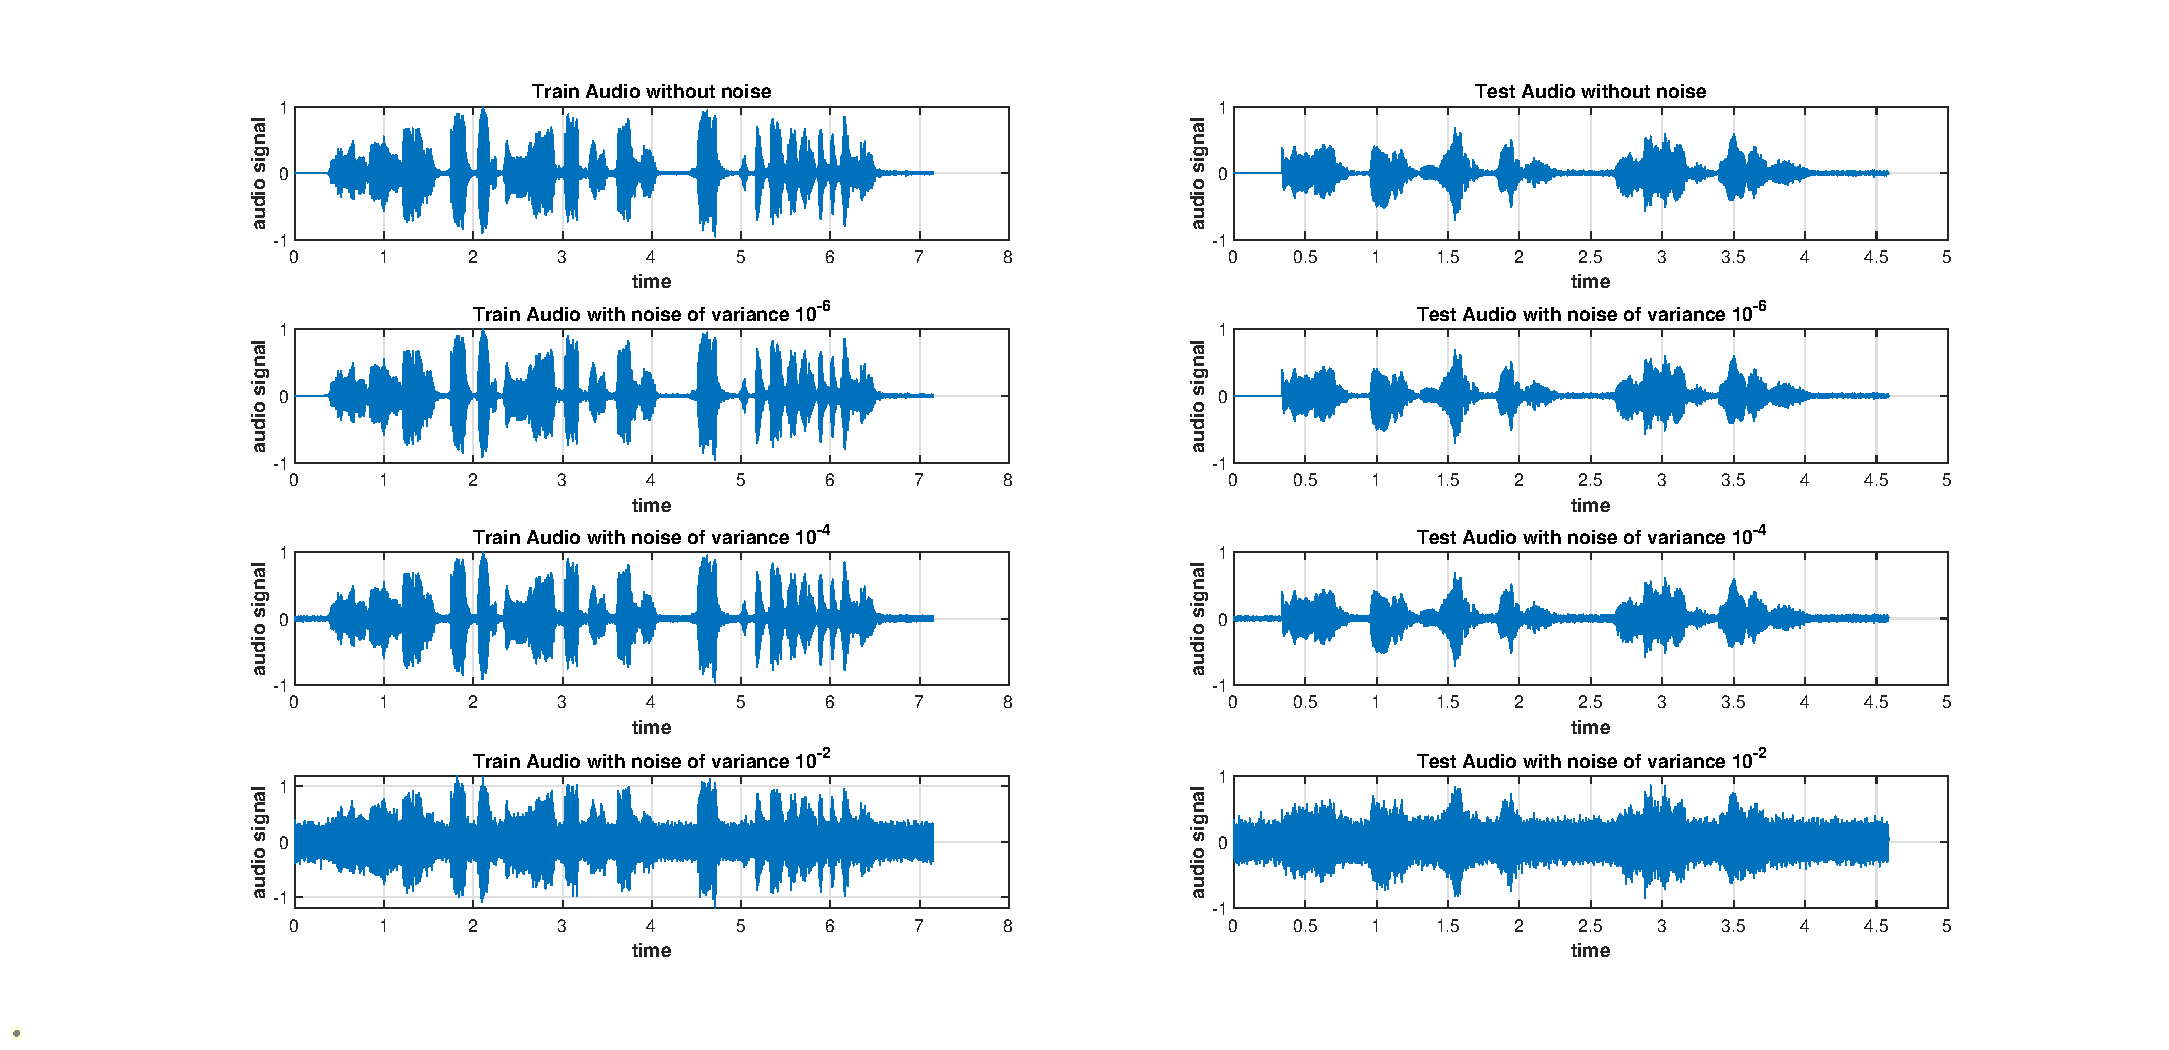
\includegraphics[scale=0.4]{Audio_Case-3.eps}%{Cepstrum}
%\caption{Conversion of Spectrum to Cepstrum}
%\end{center}
%\label{audiofiles2}
%\end{figure}
%
\begin{figure}[!b]
\begin{center}
%\includegraphics[scale=0.4]{audio.eps}%{Cepstrum}
%
\includegraphics[scale=0.4]{Audio_Case-2.eps}%{Cepstrum}
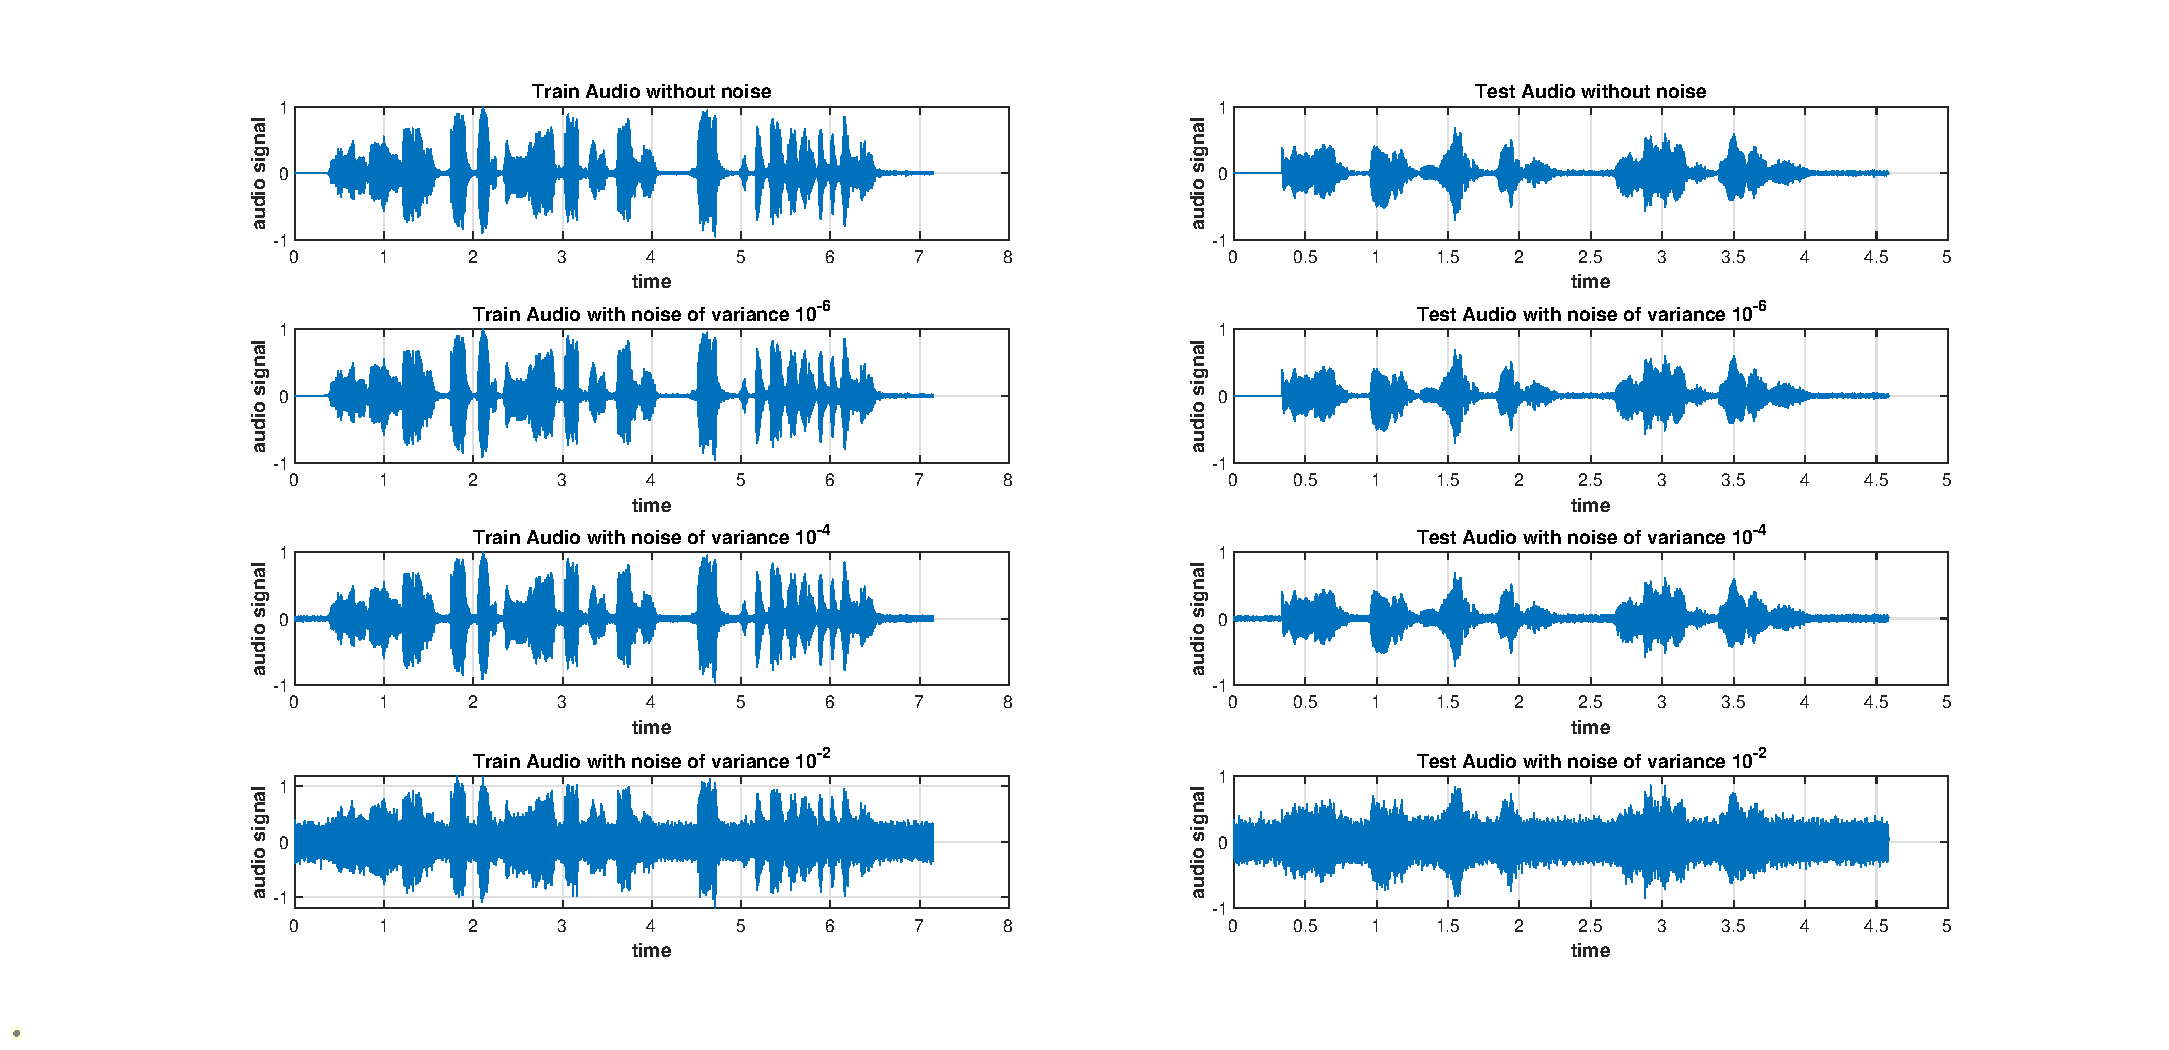
\includegraphics[scale=0.4]{Audio_Case-3.eps}%{Cepstrum}
\caption{Audio Samples: With and without noise corruption}
\label{audiofiles3}
\end{center}
\end{figure}
\newpage
In a practical situation, ambient noise may distort the voice signal and its statistical properties. Hence, in order to test the efficiency of GMMs for speaker recognition, GMMs have been trained after adding Gaussian noise with varying variances to the audio extracted from the training files and the accuracy is tested. Figure \ref{audiofiles3} shows the audio noise samples with and without Gaussian noise corruption for varying noise variance. % for a case of noise of particular variance. 
The noise variance versus accuracy is tablulated in the following for three different cases:\\
a) Only Training files are corrupted with additive noise\\
b) Testing files corrupted with additive noise and \\
c) Both training and testing files corrupted with noise.

\begin{table}[!h]
\centering
\begin{tabular}{|c|c|}
\hline
\multicolumn{1}{|l|}{Variance of Noise} & \multicolumn{1}{l|}{Accuracy(in \%)} \\ \hline
$10^{-10}$               & 100                                 \\ \hline
$10^{-8}$                & 92.59                               \\ \hline
$10^{-6}$                & 81.48                               \\ \hline
$10^{-5}$                & 59.25                               \\ \hline
$10^{-4}$                & 37.03                               \\ \hline
$10^{-2}$                & 22.22                               \\ \hline
$1$                       & 7.407                              \\ \hline
\end{tabular}
\caption{Accuracy of Speaker Recognition for varying noise variance: Noise corruption of training files}
\label{Table1}
\end{table}

\begin{table}[!h]
\centering
\begin{tabular}{|c|c|}
\hline
\multicolumn{1}{|l|}{Variance of Noise} & \multicolumn{1}{l|}{Accuracy(in \%)} \\ \hline
$10^{-10}$               & 100                                 \\ \hline
$10^{-8}$                & 92.59                               \\ \hline
$10^{-6}$                & 66.66                               \\ \hline
$10^{-5}$                & 62.96                               \\ \hline
$10^{-4}$                & 59.26                               \\ \hline
$10^{-2}$                & 14.80                               \\ \hline
$1$                       & 11.11                              \\ \hline
\end{tabular}
\caption{Accuracy of Speaker Recognition for varying noise variance: Noise corruption of testing files}
\label{Table2}
\end{table}

\begin{table}[!h]
\centering
\begin{tabular}{|c|c|}
\hline
\multicolumn{1}{|l|}{Variance of Noise} & \multicolumn{1}{l|}{Accuracy(in \%)} \\ \hline
$10^{-10}$               & 100                                 \\ \hline
$10^{-8}$                & 100                               \\ \hline
$10^{-6}$                & 96.29                               \\ \hline
$10^{-5}$                & 96.29                               \\ \hline
$10^{-4}$                & 88.88                               \\ \hline
$10^{-2}$                & 70.37                               \\ \hline
$1$                       & 25.92                              \\ \hline
\end{tabular}
\caption{Accuracy of Speaker Recognition for varying noise variance: Noise corruption of both training and test files}
\label{Table3}
\end{table}

%The Gaussian noise has been added to the audio samples of each speaker by creating noise using \textit{numpy.random.normal}(mean,std\_dev,audio) in python. If it is considered that $\bm y$ is the output signal with $\bm x$ as the input signal and $\bm n$ as the additional Gaussian noise, then:
%\begin{equation}
%\bm y = \bm x + \bm n
%\end{equation} 

From the Table \ref{Table1} , \ref{Table2} and \ref{Table3}, the efficiency of GMM in Speaker Recognition system may be inferred as follows: When the noise variance increases, the accuracy of detection gradually decreases. %which can be explained on the basis of the {Signal-to-Noise Ratio} (i.e., SNR). 
It was observed that the average power of each of the audio samples used for training were observed to be very low. As a result, for some speakers the noise with variances above the audio signal power, the GMMs could not be trained properly, which in turn lead to loss in accuracy. %Due to this, speaker recognition for some of the speech samples in testing phase could not function, thus, leading to accuracy decreasing below $50\%$.

\textcolor{black}{
%It is observed that GMM based SR is highly accurate (100$\%$ approx). %, if the approach of \textbf{GMM-ML} for \textbf{Speaker Recognition} is used. 
Hence, it may be concluded that GMM-ML approach for accomplishing Speaker Recognition (SR) is highly efficient and can be used in practical applications where SR is important.}

\section{\textbf{{A Few Conclusive Remarks on Work Done}}}
\label{conclusion}
%I would like to conclude this report by stating that, the 
\textit{Machine Learning} is a holistic approach which renders \textit{Speaker} Recognition efficient when compared to \textit{Speech} Recognition methods for Speaker idenfitication applications. %Hence, \textbf{Machine Learning} helps us to achieve the goal of Speaker Recognition and makes us understand about differences between \textit{Speaker Recognition} \& \textit{Speech Recognition}.
%As discussed in section \ref{result}, the results which are obtained when the python codes are executed, are observed to be quite accurate, which concludes that the \textit{GMM-ML} approach can be a highly efficient solution for achieving \textit{Speaker Recognition }(SR) practically.
In this work, performance of GMM-ML is studied for classifying active speaker identification problem, for both clean speech and speech corrupted with additive Gaussian noise. \textcolor{black}{It is observed that, for clean speech $100\%$ accuracy may be achieved when tested over 10 different speakers. However, when the training and testing files were corrupted with additive Gaussian noise, the accuracy of speaker recognition decreased with increasing noise variance. }}
%\bibliographystyle{plain}
\begin{thebibliography}{1}
\bibitem{1}J. Meng, J. Zhang and H. Zhao, "Overview of the Speech Recognition Technology," 2012 Fourth International Conference on Computational and Information Sciences, 2012, pp. 199-202, doi: 10.1109/ICCIS.2012.202.
\bibitem{2} T. B. Mokgonyane, T. J. Sefara, T. I. Modipa, M. M. Mogale, M. J. Manamela and P. J. Manamela, "Automatic Speaker Recognition System based on Machine Learning Algorithms," 2019 Southern African Universities Power Engineering Conference/Robotics and Mechatronics/Pattern Recognition Association of South Africa (SAUPEC/RobMech/PRASA), 2019, pp. 141-146, doi: 10.1109/RoboMech.2019.8704837.
\bibitem{3}O. M. M. Mohamed and M. Jaïdane-Saïdane, "Generalized Gaussian mixture model," 2009 17th European Signal Processing Conference, 2009, pp. 2273-2277.
\bibitem{4}L. Li, Y. Wu, Y. Ou, Q. Li, Y. Zhou and D. Chen, "Research on machine learning algorithms and feature extraction for time series," 2017 IEEE 28th Annual International Symposium on Personal, Indoor, and Mobile Radio Communications (PIMRC), 2017, pp. 1-5, doi: 10.1109/PIMRC.2017.8292668. 
\bibitem{5}Kotz, S. \& Balakrishnan, N. \& Johnson, N.L.. (2005). Continuous Multivariate Distributions, Models and Applications: Second Edition. 10.1002/9780471722069. 
\bibitem{6}T. K. Moon, "The expectation-maximization algorithm," in IEEE Signal Processing Magazine, vol. 13, no. 6, pp. 47-60, Nov. 1996, doi: 10.1109/79.543975.
\bibitem{7}Z. Wanli and L. Guoxin, "The research of feature extraction based on MFCC for speaker recognition," Proceedings of 2013 3rd International Conference on Computer Science and Network Technology, 2013, pp. 1074-1077, doi: 10.1109/ICCSNT.2013.6967289.
\bibitem{8}R. Vergin and D. O'Shaughnessy, "Pre-emphasis and speech recognition," Proceedings 1995 Canadian Conference on Electrical and Computer Engineering, 1995, pp. 1062-1065 vol.2, doi: 10.1109/CCECE.1995.526613.
\bibitem{9}M. Sahidullah and G. Saha, "A Novel Windowing Technique for Efficient Computation of MFCC for Speaker Recognition," in IEEE Signal Processing Letters, vol. 20, no. 2, pp. 149-152, Feb. 2013, doi: 10.1109/LSP.2012.2235067.
\bibitem{10}S. K. Kopparapu and M. Laxminarayana, "Choice of Mel filter bank in computing MFCC of a resampled speech," 10th International Conference on Information Science, Signal Processing and their Applications (ISSPA 2010), 2010, pp. 121-124, doi: 10.1109/ISSPA.2010.5605491.
\end{thebibliography}

\end{document}